\section{Bisimulation equivalence}
% no \IEEEPARstart
Bisimulation equivalence (bisimilarity)\footnote{The notion of bisimulation equivalence (bisimilarity) in this chapter 
refers to strong bisimulation equivalence (strong bisimilarity)} is a binary relation between labeled transition systems 
which associates systems that can simulate each other's behaviour in a stepwise manner. This enables comparison of 
different transition systems. An alternative perspective is to consider bisimulation equivalence as a relation between 
states of a single labelled transition system. By considering the quotient transition system under such a relation, smaller 
models are obtained \cite{ModelChecking}.

The bisimulation equivalence finds its extensive application in the area of formal verification of concurrent systems,
for example to check the equivalence of an implementation of a certain system with respect to its specification model.

In our tool the process of determining an existance of a bisimulation equivalence 
between two labeled transition systems was implemented using an approach which consists of three steps:
\begin{enumerate}
\item Computing strong bisimulation equivalence (strong bisimilarity) for each of the two LTSs;
\item Minimizing each of the two LTSs to its canonical form using the strong bisimilarity obtained
in the first step;
\item Performing a comparison between the two canonical forms obtained in the second step.
\end{enumerate}

The first step, computing strong bisimulation equivalence, was implemented with two different methods: the so called
naive method and a more efficient method due to Fernandez, both of which can serve as minimization procedures.

The naive algorithm \cite{ReactiveSystems1} for computing bisimulation equivalence stems from the theory underlying 
Tarski's fixed point theorem \cite{ReactiveSystems2}. It has been proven that the strong bisimulation equivalence is 
the largest fixed point of the monotic function $F$ as defined in \cite{ReactiveSystems1} given by Tarsky's fixed 
point theorem. 

The labeled graph was represented as a list of nodes and the following terminology was used:
\begin{itemize}
	\item $S_p=\{(a, q)\}$ - set of pairs $(a, q)$ for state $p$ where $a$ is an outgoing action for $p$ and $q$ is a state
	reachable from $p$ with the action $a$
\end{itemize}

Our Java implementation the algorithm takes as input an LTS in aldebaran format, generates a corresponding labeled 
graph and then computes the strong bisimulation equivalence as pairs of bisimilar states.

This algorithm has time complexity of $O(mn)$ for a labeled transition system with \emph{m} transitions and \emph{n} 
states. 

The algorithm due to Fernandez exploits the idea of the relationship between strong bisimulation equivalence 
and the relational coarsest partition problem solved by Paige and Tarjan. It represents adaptation of the 
Paige-Tarjan algorithm of complexity $O(m \log n)$ to minimize labeled transition systems modulo bisimulation 
equivalence by computing the coarsest partition problem with respect to the family of binary relations 
$\left(T_a\right)_{a\in A}$ instead of one binary relation, where $T_a=\{(p,q)|(p,a,q)\in T\}$ is a transition 
relation for action ${a\in A}$ and $T$ is a set of all transitions \cite{PaigeTarjan, Fernandez}.

The algorithm due to Fernandez in our implementation in Java takes an LTS in aldebaran format as an input, generates a 
corresponding labeled graph and then partitions the labeled graph into its coarsest blocks where each block represents 
a set of bisimilar states. Partition is a set of mutually exclusive blocks whose union constitutes the graph universe.

To define graph transitions the following terminology was used: 
\begin{itemize}
	\item $T_a[p]=\{q\}$ - an $a$-transition from state $p$ to state $q$
	\item $T_a{}^{-1}[q]=\{p\}$ - an inverse $a$-transition from state $q$ to state $p$
	\item $T_a{}^{-1}[B]=\cup \left\{T_a{}^{-1}[q],q\in B\right\}$ - inverse transition for block $B$ and action $a$
	\item $W$ - set of sets called splitters that are being used to split the partition
	\item infoB$(a, p)$ - info map for block $B$, state $p$ and action $a$
\end{itemize}

The time complexity of Fernandez's algorithm is $O(m \log n)$ for a labeled transition system 
with $m$ transitions and $n$ states. 

The next step uses the bisimulation equivalence computed in the first step in order to minimize the graphs. This reduction 
is implemented as follows:
\begin{enumerate}
	\item If a pair of states $(p, q)$ is bisimilar, then the two states are merged into one single state $k$;
	\item All incoming transitions $r \stackrel{a}{\rightarrow} p$ and $s \stackrel{a}{\rightarrow} q$ are replaced by transitions $r \stackrel{a}{\rightarrow} k$ and $s \stackrel{a}{\rightarrow} k$;
	\item All outgoing transitions $p \stackrel{a}{\rightarrow} r$ and $q \stackrel{a}{\rightarrow} s$ are replaced by transitions $k \stackrel{a}{\rightarrow} r$ and $k \stackrel{a}{\rightarrow} s$;
	\item The duplicate transitions are not taken into consideration.
\end{enumerate}
The procedure is repeated for all pairs of bisimilar states.

Having reduced the two labeled graphs into their minimal forms, the last step in the process of checking the equivalence
between the two labeled transition systems consists of checking whether the two minimal labeled graphs are isomorphic.
Two isomorphic graphs are always bisimilar \cite{HandbookProcessAlgebra2}.

Two graphs $G$ and $H$ are isomorphic if there exists a graph isomorphism between them. According to \cite{HandbookProcessAlgebra1}, 
a graph isomorphism between two graphs G and H is a bijective function $f: Nodes(G) \rightarrow Nodes(H)$ satisfying:
\begin{itemize}
	\item $f(initialNode(G)) = g(initialNode(H))$
	\item $(s, a, t)$ is an edge in $G \Leftrightarrow (f(s), a, f(t))$ is an edge in $H$
\end{itemize}

The graph isomorphism check was implemented recursively as follows: Starting from the initial states of the minimal graphs, 
the outgoing labeled transitions have to be same, and for every outgoing transition with a given label in the first graph, 
there has to be another one in the other graph with the same label that leads again to isomorphic states. 

The process of determining equivalence of two labeled transition systems with respect to strong bisimularity is illustrated 
on the graphs Graph 1 and Graph 2 as input labeled graphs.
\begin{figure}[h!]
\centering
\subfigure[Graph 1]{
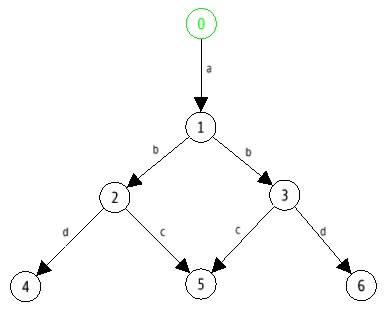
\includegraphics[width=2.3in]{graph1}
\label{fig:graph1}
}
\subfigure[Graph 2]{
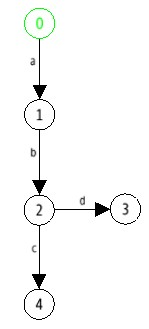
\includegraphics[width=0.9in]{graph2}
\label{fig:graph2}
}
\label{fig:exampleGraphs}
\caption{Example of two labeled graphs}
\end{figure}

The result from the first step, computing the strong bisimulation equivalence, is given in TABLE \ref{table1} for both the
naive algorithm and the advanced algorithm due to Fernandez:
\begin{table}[h!]
\begin{tabular}{| l | p{3.2cm}| p{3.2cm} | }
  \hline                       
  Algorithm & Graph 1 & Graph 2 \\ \hline
  Naive & \{(2, 3), (3, 2), (4, 5), 
(5, 4), (4, 6), (6, 4), (5, 6), (6, 5), (0, 0), (1, 1), (2, 2), (3, 3), (4, 4), (5, 5), (6, 6)\} & \{(3, 4), (4, 3), (0, 0), 
(1, 1), (2, 2), (3, 3), (4, 4)\} \\ \hline
  Fernandez & \{\{0\}, \{1\}, \{2\}, \{3\}, \{4, 5, 6\}\} & \{\{0\}, \{1\}, \{2\}, \{3, 4\}\} \\ \hline  
\end{tabular}
\caption{Computing strong bisimularity for Graph 1 and Graph 2}
\label{table1}
\end{table}

The second step involves minimization of the input graphs using the bisimulation equivalence obtained in the first step. 

The process of reduction of Graph 1 to its minimal form is given on Fig. \ref{fig:bisimGraph1}. As it can be seen from the figure, 
all mutually bisimilar states are merged into a single state: the states 2 and 3 are merged into state 2 in the minimal graph, and 
states 4, 5, and 6 are merged into state 3 in the minimal graph.
\begin{figure}[h!]
\centering
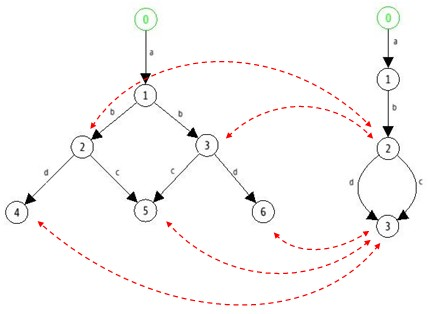
\includegraphics[width=2.8in]{bisimGraph1}.
\caption{Minimized Graph 1}
\label{fig:bisimGraph1}
\end{figure}

Similarly, Fig. \ref{fig:bisimGraph2} illustrates the process of reduction of Graph 2 to its minimal form. Here, the states 
3 and 4 are merged into state 3 in the minimal graph.
\begin{figure}[h!]
\centering
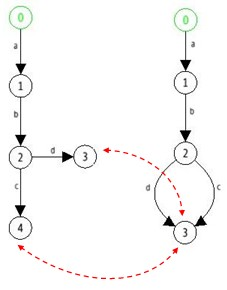
\includegraphics[width=1.6in]{bisimGraph2}
\caption{Minimized Graph 2}
\label{fig:bisimGraph2}
\end{figure}

In the last step, the two minimal graphs from \ref{fig:bisimGraph1} and \ref{fig:bisimGraph2} are compared for graph isomorphism.
From the figures, it can be seen that the minimal graphs are isomorhic which implies that the two input graphs Graph 1 and Graph 2 
are bisimular and they exhibit the same behaviour.

The correctness of the implementation was tested with the use of ltsconvert and ltscompare tools of mCRL2, micro Common Representation Language 2, a specification language that can be used to specify and analyse the behaviour of distributed systems and protocols
\cite{mCRL2Ref}.